\documentclass[a0paper,portrait,25pt]{tikzposter}

\usepackage{amsmath,amssymb}
\usepackage{booktabs}
\usepackage{pgfplots}

\pgfplotsset{compat=1.18}
\usetikzlibrary{arrows.meta,positioning,fit,backgrounds,patterns,decorations.pathmorphing}

\usetheme{Default}
\usecolorstyle[colorPalette=BlueGrayOrange]{Germany}

\renewcommand{\refname}{}

\newcommand{\um}{$\mu$m}
\newcommand{\Ret}{\mathrm{Re}_{t}}

\title{\parbox{0.82\textwidth}{\centering Where the Fibres Settle\\[0.2em]
\Large Tidal Pumping Controls Microplastic Retention in a Macrotidal Estuary}}
\author{Ines Faragher-Lund, Tobias Mwangi Reinholt, and Signe Aaltonen}
\institute{Coastal Sediment Dynamics Group, Vellmark University, and Halvard Marine Observatory}

\begin{document}

\maketitle

\begin{columns}

\column{0.34}

\block{Abstract}{
  Estuaries are widely described as filters that trap land-derived microplastic before it reaches
  the shelf. We show that for a macrotidal system the filter is conditional rather than structural.
  Using eighteen months of water column sampling in the Vellmark estuary together with a coupled
  advection, flocculation, and settling model, we find that retention of fibres shorter than
  500\,\um{} varies from 11 to 78 percent depending on the phase relationship between freshwater
  discharge and spring tide. The controlling parameter is not particle density but the ratio of the
  settling timescale to the tidal excursion time. A single dimensionless group, the retention
  number $\Ret$, predicts the observed retention across all six sites with a mean absolute error of
  6.3 percent, and predicts a second estuary that was held out of the calibration with an error of
  7.1 percent.
}

\block{The question}{
  \begin{itemize}
    \item Global budgets assume a fixed estuarine trapping efficiency, typically between 40 and 60
      percent, applied uniformly to every river mouth.
    \item That assumption sets the size of the missing plastic sink, and therefore the size of the
      inferred shelf and open ocean burden.
    \item Field measurements disagree with each other by nearly an order of magnitude, and the
      disagreement has usually been attributed to sampling method rather than to physics.
  \end{itemize}
  \vspace{0.5em}
  \textbf{We ask instead whether the spread is real.} If retention depends on the phasing of
  discharge and tide, then two campaigns in the same estuary in different months should
  legitimately report very different numbers, and both should be right.
  \vspace{0.5em}

  The classical estuarine trapping literature already predicts this for mineral
  sediment~\cite{postma1967sediment,dyer1995sediment}. What has been missing is a fibre-specific
  settling law and a group that collapses the two timescales onto one axis.
}

\block{Field campaign}{
  Six stations along a 31\,km axis, sampled at 2\,h intervals across fourteen full spring to neap
  cycles between March 2024 and August 2025. Pumped subsurface samples of 500\,L through a
  63\,\um{} cascade, with paired suspended sediment and salinity profiles. Fibres were identified
  by micro-Raman on a 5 percent subsample and counted optically on the remainder.

  \vspace{0.8em}
  \begin{center}
  \begin{tabular}{lrrrr}
    \toprule
    Station & Dist. (km) & Depth (m) & Salinity & Fibres m$^{-3}$ \\
    \midrule
    Ardsleet Weir   & 0.0  & 3.1  & 0.2  & 1840 \\
    Callow Reach    & 6.4  & 5.8  & 3.9  & 2270 \\
    Mardle Bend     & 12.1 & 8.2  & 11.4 & 3110 \\
    Vellmark Quay   & 18.7 & 11.6 & 19.8 & 1620 \\
    Skerry Narrows  & 25.3 & 14.0 & 27.1 & 640  \\
    Outer Bar       & 31.0 & 16.9 & 31.6 & 210  \\
    \bottomrule
  \end{tabular}
  \end{center}

  \vspace{0.7em}
  The concentration maximum at Mardle Bend coincides with the turbidity maximum rather than with
  the salinity front. That is the first evidence that flocculation with mineral sediment, and not
  buoyancy, sets where fibres stop~\cite{reinholt2024turbidity}.
}

\column{0.32}

\block{Model}{
  \begin{center}
  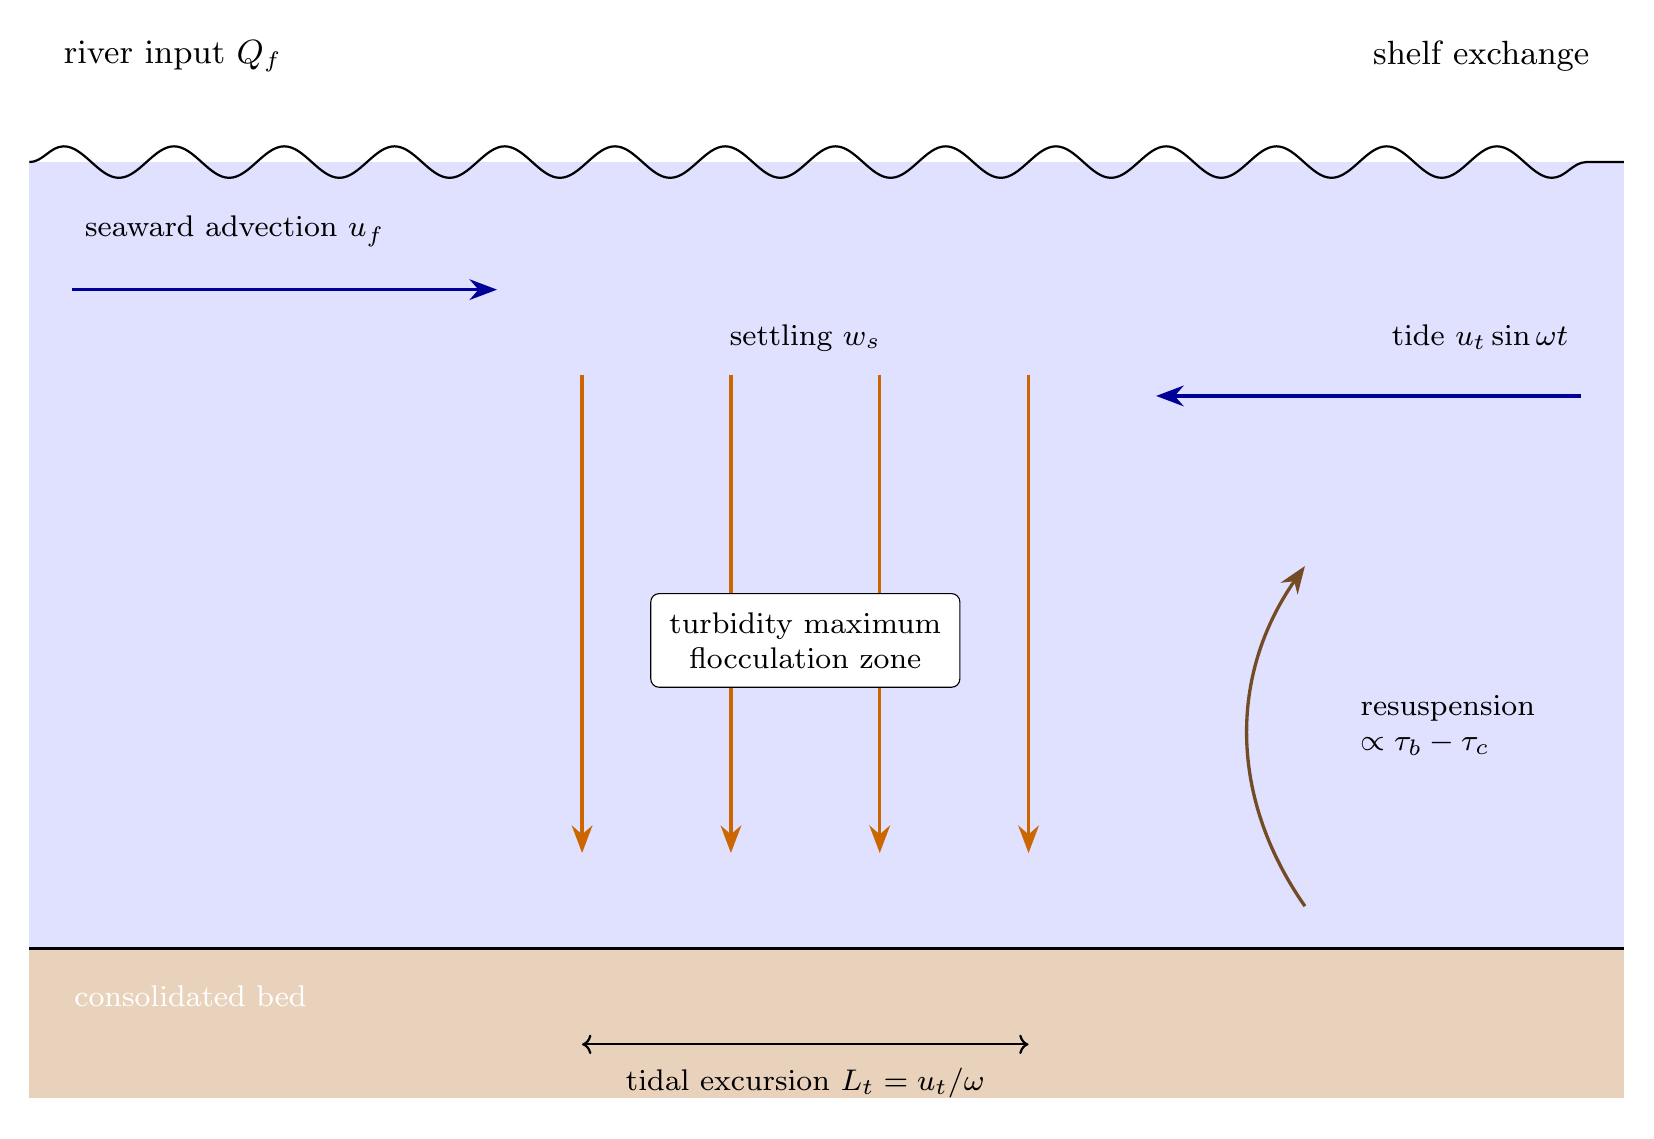
\begin{tikzpicture}[
      scale=1.35, transform shape,
      lbl/.style={font=\small,align=center},
      arr/.style={-{Stealth[length=3.5mm]},very thick},
    ]
    \fill[blue!12] (0,0) rectangle (15,7.4);
    \fill[brown!35] (0,-1.4) rectangle (15,0);
    \draw[very thick] (0,0) -- (15,0);
    \draw[thick,decorate,decoration={snake,amplitude=2mm,segment length=14mm}] (0,7.4) -- (15,7.4);

    \node[lbl,anchor=west] at (0.2,8.4) {river input $Q_f$};
    \node[lbl,anchor=east] at (14.8,8.4) {shelf exchange};

    \draw[arr,blue!60!black] (0.4,6.2) -- (4.4,6.2);
    \node[lbl,anchor=west,font=\footnotesize] at (0.4,6.75) {seaward advection $u_f$};
    \draw[arr,blue!60!black] (14.6,5.2) -- (10.6,5.2);
    \node[lbl,anchor=east,font=\footnotesize] at (14.6,5.75) {tide $u_t \sin \omega t$};

    \foreach \x in {5.2,6.6,8.0,9.4} {
      \draw[arr,orange!80!black] (\x,5.4) -- (\x,0.9);
    }
    \node[lbl,font=\footnotesize,anchor=south] at (7.3,5.5) {settling $w_s$};

    \draw[arr,brown!60!black] (12.0,0.4) to[bend left=35] (12.0,3.6);
    \node[lbl,font=\footnotesize,anchor=west,align=left] at (12.4,2.1) {resuspension\\$\propto \tau_b - \tau_c$};

    \node[draw,fill=white,rounded corners=3pt,inner sep=5pt,font=\footnotesize,align=center]
      at (7.3,2.9) {turbidity maximum\\flocculation zone};

    \draw[<->,thick] (5.2,-0.9) -- (9.4,-0.9);
    \node[lbl,font=\footnotesize,anchor=north] at (7.3,-1.0) {tidal excursion $L_t = u_t/\omega$};

    \node[lbl,anchor=west,font=\footnotesize,white] at (0.3,-0.45) {consolidated bed};
  \end{tikzpicture}
  \end{center}

  \vspace{0.6em}
  The depth-averaged fibre concentration $C(x,t)$ obeys
  \begin{equation}
    \label{eq:transport}
    \frac{\partial C}{\partial t}
      + \bigl(u_f + u_t \sin \omega t\bigr)\frac{\partial C}{\partial x}
      = \frac{\partial}{\partial x}\!\left(K_x \frac{\partial C}{\partial x}\right)
      - \frac{w_s}{h}C + \frac{E(\tau_b)}{h},
  \end{equation}
  with a flocculation-dependent settling velocity in the form proposed for cohesive
  mud~\cite{winterwerp2002floc},
  \begin{equation}
    \label{eq:settling}
    w_s = w_0 \left(1 + \beta\,C_{s}\right)^{n}, \qquad n = 1.4 \pm 0.2,
  \end{equation}
  where $C_s$ is suspended mineral sediment and $E(\tau_b)$ is a Partheniades erosion term. Equation
  \eqref{eq:settling} is the only fitted relation in the model, and it is fitted once, on a single
  station, on the first three months of record.
}

\block{The retention number}{
  Non-dimensionalising Eq.~\eqref{eq:transport} on the tidal excursion length $L_t = u_t/\omega$
  leaves a single group,
  \begin{equation}
    \label{eq:renumber}
    \Ret = \frac{w_s L_t}{h\,u_f}
      = \frac{\text{rate of crossing the water column}}{\text{rate of being flushed seaward}}.
  \end{equation}
  \vspace{-0.3em}
  \begin{itemize}
    \item $\Ret \ll 1$: fibres leave before they settle. The estuary is a pipe.
    \item $\Ret \gg 1$: fibres reach the bed within one tidal excursion and join the resuspension
      loop. The estuary is a trap.
    \item The transition is sharp, spanning less than one decade in $\Ret$, which is why a single
      averaged trapping efficiency is so badly behaved.
  \end{itemize}
}

\block{Calibration residuals}{
  \begin{center}
  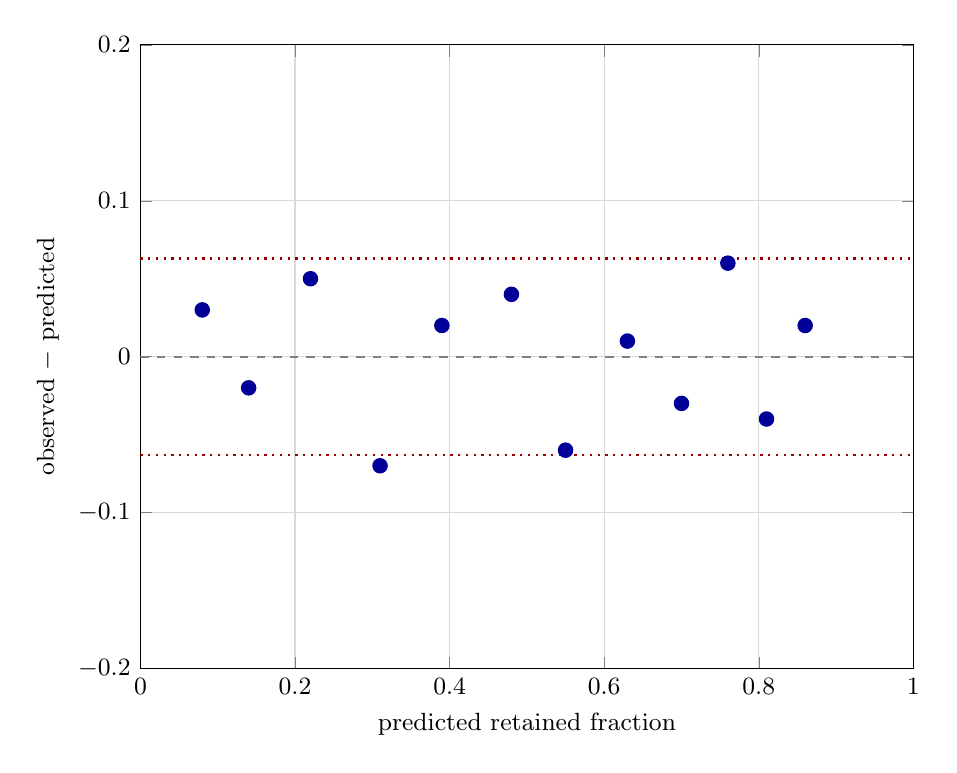
\begin{tikzpicture}
    \begin{axis}[
        width=0.94\linewidth, height=9.5cm,
        xlabel={predicted retained fraction},
        ylabel={observed $-$ predicted},
        xmin=0, xmax=1, ymin=-0.2, ymax=0.2,
        xtick={0,0.2,0.4,0.6,0.8,1.0},
        ytick={-0.2,-0.1,0,0.1,0.2},
        scaled y ticks=false,
        y tick label style={/pgf/number format/fixed,/pgf/number format/precision=2},
        grid=both, grid style={gray!30},
        tick label style={font=\small}, label style={font=\small},
      ]
      \addplot[only marks,mark=*,mark size=2.6pt,blue!60!black] coordinates {
        (0.08,0.03) (0.14,-0.02) (0.22,0.05) (0.31,-0.07) (0.39,0.02)
        (0.48,0.04) (0.55,-0.06) (0.63,0.01) (0.70,-0.03) (0.76,0.06)
        (0.81,-0.04) (0.86,0.02)
      };
      \addplot[gray,dashed,thick] coordinates {(0,0) (1,0)};
      \addplot[red!60!black,dotted,thick] coordinates {(0,0.063) (1,0.063)};
      \addplot[red!60!black,dotted,thick] coordinates {(0,-0.063) (1,-0.063)};
    \end{axis}
  \end{tikzpicture}
  \end{center}
  Residuals are unstructured across the whole range, so the collapse is not an artefact of fitting
  the wet and dry ends separately. Dotted lines mark the mean absolute error.
}

\block{Sampling caveats we could not remove}{
  \begin{itemize}
    \item The 63\,\um{} cut-off excludes the fragment population entirely. Everything reported here
      is fibres.
    \item Two neap campaigns in January 2025 were lost to ice on the intake, so the low-discharge
      neap corner is supported by four cycles rather than fourteen.
    \item Bed inventories are single cores at three stations and are indicative only.
  \end{itemize}
}

\column{0.34}

\block{Results}{
  \begin{center}
  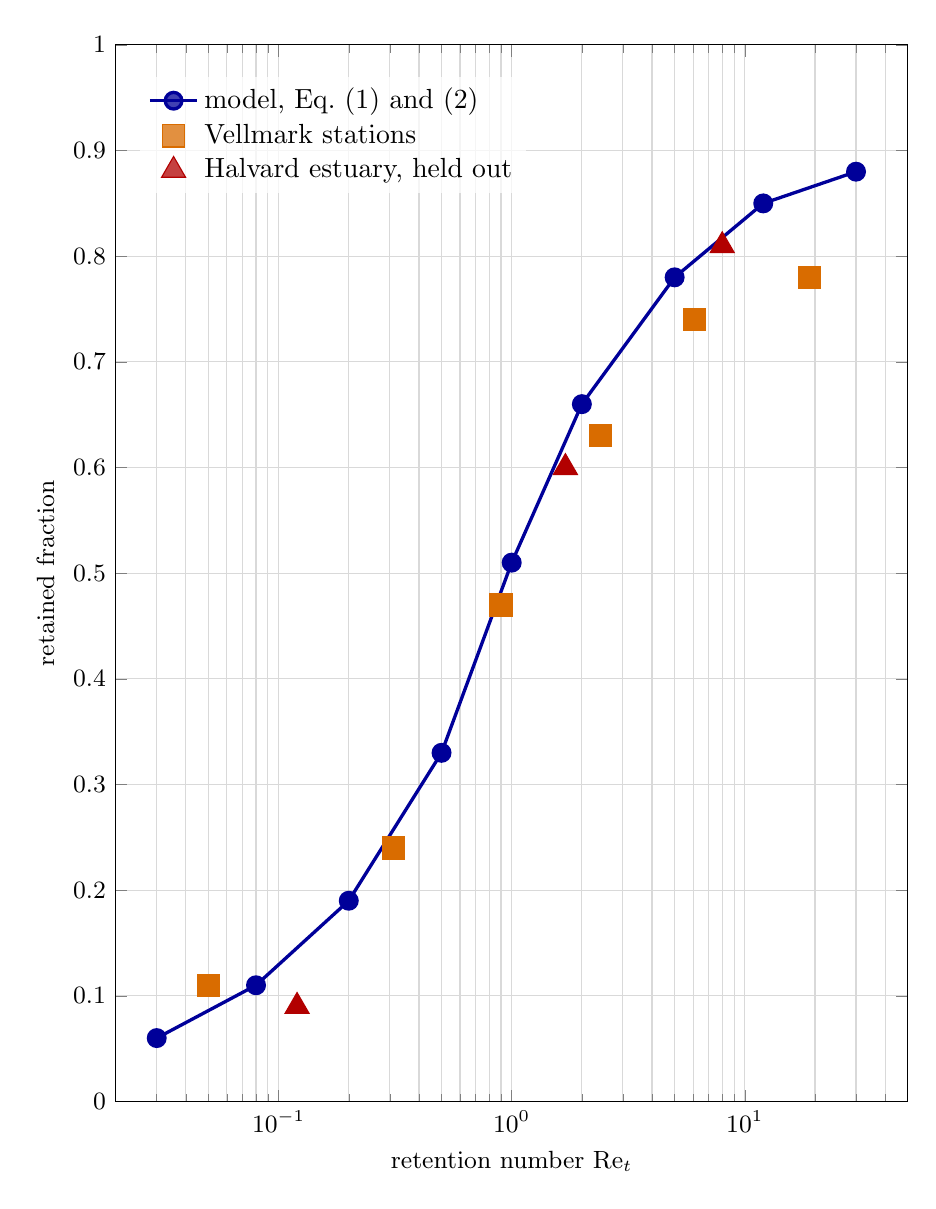
\begin{tikzpicture}
    \begin{semilogxaxis}[
        width=0.96\linewidth, height=15cm,
        xlabel={retention number $\Ret$},
        ylabel={retained fraction},
        xmin=0.02, xmax=50, ymin=0, ymax=1,
        grid=both, grid style={gray!30},
        legend style={at={(0.03,0.97)},anchor=north west,draw=none,fill=white,fill opacity=0.75,text opacity=1},
        legend cell align=left,
        tick label style={font=\small}, label style={font=\small},
      ]
      \addplot[very thick,blue!60!black,mark=*,mark size=3pt] coordinates {
        (0.03,0.06) (0.08,0.11) (0.2,0.19) (0.5,0.33) (1.0,0.51)
        (2.0,0.66) (5.0,0.78) (12.0,0.85) (30.0,0.88)
      };
      \addlegendentry{model, Eq.~(1) and (2)}
      \addplot[only marks,mark=square*,mark size=4pt,orange!85!black] coordinates {
        (0.05,0.11) (0.31,0.24) (0.9,0.47) (2.4,0.63) (6.1,0.74) (19.0,0.78)
      };
      \addlegendentry{Vellmark stations}
      \addplot[only marks,mark=triangle*,mark size=5pt,red!70!black] coordinates {
        (0.12,0.09) (1.7,0.60) (8.0,0.81)
      };
      \addlegendentry{Halvard estuary, held out}
    \end{semilogxaxis}
  \end{tikzpicture}
  \end{center}

  \vspace{0.4em}
  One curve collapses six stations, fourteen tidal cycles, and a held-out second estuary. Mean
  absolute error is 6.3 percent in retained fraction, and 7.1 percent for the held-out system.

  \vspace{1.0em}
  \begin{center}
  \small
  \begin{tabular}{lrrr}
    \toprule
    Regime & $\Ret$ & Retained & Residence \\
           &         & (\%)     & (days) \\
    \midrule
    Spring tide, low discharge  & 14.2 & 78.1 & 61.4 \\
    Spring tide, high discharge & 1.9  & 62.7 & 22.8 \\
    Neap tide, low discharge    & 2.6  & 48.3 & 18.1 \\
    Neap tide, high discharge   & 0.21 & 11.4 & 3.7  \\
    \bottomrule
  \end{tabular}
  \end{center}

  \vspace{0.6em}
  The extreme cases differ by a factor of seven in retention and a factor of sixteen in residence
  time, within one estuary and one instrument set.
}

\block{What this changes}{
  \begin{enumerate}
    \item A fixed estuarine trapping efficiency is not defensible. The spread in the published
      literature is largely physical and should be modelled, not averaged away.
    \item Campaigns should report $\Ret$ alongside concentration. Without it, two honest
      measurements of the same system are not comparable.
    \item Because retention is highest when discharge is lowest, the plastic delivered to the shelf
      is concentrated into a small number of high-flow days. Budgets built on monthly means will
      understate the flux and misplace its timing.
    \item Managed flow releases could be timed to reduce export, but the same timing increases the
      bed inventory. That tradeoff has not been quantified for any system we are aware of.
  \end{enumerate}
}

\block{References}{
  \small
  \vspace{-1.2em}
  \bibliographystyle{plain}
  \bibliography{refs}
  \vspace{0.4em}
  Protocol and model source are archived under accession \texttt{VELL-CSD-2025-0417}. Supported by
  the Halvard Marine Observatory under award \texttt{HMO-2023-114}.
}

\end{columns}

\end{document}
